\documentclass{article}
\usepackage[utf8]{inputenc}
\usepackage[margin=1in]{geometry}
\usepackage{hyperref}
\usepackage{setspace}
\pagenumbering{arabic}
\usepackage{graphicx}
\usepackage[dvipsnames]{xcolor}
\usepackage{fancyhdr} 
\usepackage{amsmath, amsfonts, amsthm, amssymb}
\usepackage{bbm}
\usepackage{nth}
\usepackage{dsfont}
\usepackage{subfig}
\usepackage{tikz}
\usepackage{accents}


% commenting
\newcommand{\comment}[3]{\textcolor{#1}{\textbf{[#2: }\textit{#3}\textbf{]}}}
\newcommand{\emma}[1]{\comment{purple}{EK}{#1}}
\newcommand{\jesse}[1]{\comment{BurntOrange}{JG}{#1}}
\newcommand{\miaoshiqi}[1]{\comment{ForestGreen}{ML}{#1}}
\newcommand{\siyue}[1]{\comment{blue}{SY}{#1}}

%For references using Lemma, Theorem, etc, use \cref
\usepackage[nameinlink,capitalize,sort]{cleveref}

% theorems
\newtheorem{theorem}{Theorem}[section]
\newtheorem{lemma}[theorem]{Lemma}
\newtheorem{definition}[theorem]{Definition}
\newtheorem{proposition}[theorem]{Proposition}
\newtheorem{example}[theorem]{Example}
\newtheorem{corollary}[theorem]{Corollary}
%theoremstyle{plain} %boldface title, italicized body. Commonly used in theorems, lemmas, corollaries, propositions and conjectures.
%\theoremstyle{definition} %boldface title, Roman body. Commonly used in definitions, conditions, problems and examples
\theoremstyle{remark} %italicized title, Roman body. Commonly used in remarks, notes, annotations, claims, cases, acknowledgments and conclusions.
\newtheorem{exercise}[theorem]{Exercise}

\newenvironment{solution}
  {\renewcommand\qedsymbol{$\blacksquare$}\begin{proof}[Solution]}
  {\end{proof}}

% weird hack to get rid of dot:
\usepackage{xpatch}
\makeatletter
\AtBeginDocument{\xpatchcmd{\@thm}{\thm@headpunct{.}}{\thm@headpunct{}}{}{}}



% lin alg
\newcommand{\bu}{{\mathbf{u}}}
\newcommand{\bv}{{\mathbf{v}}}
\newcommand{\bw}{{\mathbf{w}}}
\newcommand{\bx}{\mathbf{x}}
\newcommand{\zerovec}{{\mathbf{0}}}

% other useful stuff
\newcommand{\Id}{{\mathds{1}}}
\newcommand{\N}{{\mathbb{N}}}
\newcommand{\R}{{\mathbb{R}}}
\newcommand{\C}{{\mathbb{C}}}
\newcommand{\Z}{{\mathbb{Z}}}
\newcommand{\Q}{{\mathbb{Q}}}
\newcommand{\F}{{\mathbb{F}}}
\newcommand{\cL}{{\mathcal{L}}}
\newcommand{\cP}{\mathcal{P}}
\newcommand{\inv}{{-1}}

%\DeclareMathOperator{\dim}{dim}
\DeclareMathOperator{\range}{range}
\DeclareMathOperator{\rank}{rank}
\DeclareMathOperator{\nullity}{nullity}

\hypersetup{
  colorlinks   = true, %Colours links instead of boxes
  urlcolor     = blue, %Colour for external hyperlinks
  linkcolor    = black, %Colour of internal links
  citecolor   = black %Colour of citations
}

\allowdisplaybreaks % fixes align environment weird spacing on page
\setlength{\parindent}{0cm}
\usepackage[parfill]{parskip}

% get rid of dot after theorem 
\usepackage{xpatch}
\makeatletter
% Patch to accommodate for \begin{theorem}[...]
\AtBeginDocument{\xpatchcmd{\cref@thmoptarg}{\thm@headpunct{.}}{\thm@headpunct{}}{}{}}
% Patch to accommodate \begin{theorem} (without an optional argument)
\AtBeginDocument{\xpatchcmd{\cref@thmnoarg}{\thm@headpunct{.}}{\thm@headpunct{}}{}{}}


% \usepackage[natbib=true, style=vancouver]{biblatex}
 %\usepackage[backend= biber, style=alphabetic]{biblatex}
 \usepackage{natbib}
 \setcitestyle{square}
%\bibliography{references.bib}

\title{Mathematics Bootcamp Lecture Notes \\
\vspace{0.5em}
\large Department of Statistical Sciences, University of Toronto}
\author{Emma Kroell}
\date{Last updated: \today}

\begin{document}

\maketitle


\newpage
\section*{Preface}

These lecture notes were prepared for the Mathematics course at the inaugural Department of Statistical Sciences Graduate Student Bootcamp at the University of Toronto. The course teaches an overview of necessary mathematics prerequisites to incoming statistics graduate students, with an emphasis on proofs.


These lectures are based on the following books or lecture notes:

1. \href{https://link-springer-com.myaccess.library.utoronto.ca/book/10.1007/978-1-4614-4265-3}{{\emph{An Introduction to Mathematical Structures and Proofs}}} by Larry J. Gerstein \\
2. \href{https://bookstore.ams.org/amstext-26/}{{\emph{The Tools of Mathematical Reasoning}}} by Tamara J. Lakins \\
3. \href{https://link-springer-com.myaccess.library.utoronto.ca/book/10.1007/0-387-28387-0}{\emph{A Taste of Topology}} by Volker Runde \\
4. \href{https://link-springer-com.myaccess.library.utoronto.ca/book/10.1007/978-3-319-17771-7}{\emph{Real Mathematical Analysis}} by Charles C. Pugh \\
5. \href{https://link-springer-com.myaccess.library.utoronto.ca/book/10.1007/978-3-319-11080-6}{{\emph{Linear Algebra Done Right}}} by Sheldon Axler \\
6. \href{https://www.math.brown.edu/streil/papers/LADW/LADW.html}{{\emph{Linear Algebra Done Wrong}}} by Sergei Treil \\
7. \href{http://84.89.132.1/~piotr/docs/RealAnalysisNotes.pdf}{\emph{Lecture notes in Mathematics for Economics and Statistics}} by Piotr Zwiernik \\
8. \href{http://www.math.uwaterloo.ca/~lwmarcou/notes/pmath351.pdf}{{\emph{Real Analysis Lecture Notes}}} by Laurent Marcoux

Chapter 1 of Gerstein (2012) and the first three chapters of Lakins (2016) are used as references for the proof technique section. Runde (2005) is the main text for the sections on set theory, metric spaces, and topology, which follow chapters 1, 2, and 3 of his book, respectively. Some additional topics come from Pugh (2015). The linear algebra content comes mostly from Axler (2015), with Treil (2017) used in some sections for an alternate perspective.

Most of the material in these notes belongs to these texts. All of these texts are available online to University of Toronto users (some to everyone).

I would like to acknowledge the assistance of Jesse Gronsbell, Stanislav Volgushev, Piotr Zwiernik, and Robert Zimmerman in developing the list of topics for the course. 

Please notify me of any typos or corrections at emma.kroell@mail.utoronto.ca .


\newpage
\tableofcontents


\newpage

{\bf A short note on notation: }

\vspace{0.5em}

$\N$ denotes the whole numbers, i.e. $\N = \{1,2,\ldots \}$

$\N_0$ denotes the non-negative integers, i.e. $\N_0 = \{0, 1,2,\ldots \}$

$\Z$ denotes the integers, i.e. $\Z = \{ \ldots, -2,-1,0,1,2,\ldots \}$

$\Q$ denotes the rational numbers, i.e. $\Q = \{ \frac{p}{q} \, | \, p, q \in \Z \text{ and } q \neq 0 \}$

$\R$ denotes the real numbers

$\C$ denotes the complex numbers



\section{Review of proof techniques}
\subsection{Propositional logic}

\emph{Propositions} are statements that could be true or false. They have a corresponding \emph{truth value}. We will use capital letters to denote propositions. For example, ``$n$ is odd'' and ``$n$ is divisible by 2'' are propositions. Let's call them $P$ and $Q$. Whether they are true or not (i.e. their truth value) depends on what $n$ is. 

We can  negate statements: $\neg P$ is the statement ``$n$ is not odd''.

 We can combine statements: 
 \begin{itemize}
 \item $P \wedge Q$ is the statement ``$n$ is odd and $n$ is divisible by 2''.
 \item $P \vee Q$ is the statement ``$n$ is odd or $n$ is divisible by 2''.
\end{itemize}
We always assume the inclusive or unless specifically stated otherwise.


\begin{example}
Here are some statements, which we want to write in propositional logic.
\begin{itemize}
              \item If it's not raining, I won't bring my umbrella.
              \item I'm a banana or Toronto is in Canada.
              \item If I pass this exam, I'll be both happy and surprised.
\end{itemize}

For the first one, let $A$ be the statement ``it's raining'' and $B$ be the statement ``I will bring my umbrella''. In logic, the statement is $\neg A \implies \neg B$.

For the second, let $C$ be the statement ``I'm a banana'' and let $D$ be the statement ``Toronto is in Canada''. We write this as $C \vee D$.

For the third, let $P$ be the statement ``I pass this exam'', let $Q$ be the statement ``I am happy'', and let $R$ be the statement ``I am surprised''. This one is written $P \implies (Q \wedge R)$.
\end{example}

\subsubsection{Truth values}

\begin{example} Write the following using propositional logic: \\
If it is snowing, then it is cold out. \\
It is snowing. \\
Therefore, it is cold out.

Solution. \\
$P \implies Q$ \\
$P$ \\
Conclusion: $Q$ \\
\end{example}

To examine if a statement is true or not, we use a truth table, where we write out all the possibilities. 

\begin{example}
The truth table for $P \implies Q$ where $P$, $Q$ are propositions is:

\begin{tabular}{|c|c| c|}
\hline
     $P$& $Q$ &  $P \implies Q$ \\ \hline
     T& T & T \\ \hline
     T & F & F \\ \hline
     F & T & T \\ \hline
     F & F & T \\ \hline
\end{tabular}
\end{example}

\subsubsection{Logical equivalence}
We say that two statements are \emph{logically equivalent} if they have the same truth tables.

\begin{example}
\label{ex:implication_table}
Let $P$, $Q$ be propositions. $P \implies Q$ is logically equivalent to $\neg P \vee Q$.
 
 
\begin{tabular}{|c|c| c|}
\hline
     $P$& $Q$ &  $P \implies Q$ \\ \hline
     T& T & T \\ \hline
     T & F & F \\ \hline
     F & T & T \\ \hline
     F & F & T \\ \hline
\end{tabular} \hspace{2cm} \begin{tabular}{|c | c | c | c|}
\hline
     $P$& $Q$ & $\neg P$ & $\neg P \vee Q$  \\ \hline
     T& T & F & T \\ \hline
     T & F & F & F \\ \hline
     F & T &  T &T \\ \hline
     F & F & T & T \\ \hline
\end{tabular}
\end{example}

\vspace{1em}

\begin{theorem}[De Morgan's Laws]
\label{thm:demorgan}
Let $P$, $Q$ be propositions.
\begin{enumerate}
    \item[(i)] $\neg (P \wedge Q)$ is logically equivalent to $\neg P \vee \neg Q$.
    \item[(ii)] $\neg (P \vee Q)$ is logically equivalent to $\neg P \wedge \neg Q$.
\end{enumerate}
\end{theorem}

Proving this is your first exercise.

The following fact is often useful.
\begin{example}
\label{ex:ifthen}
$\neg (P \implies Q)$ is logically equivalent to $P \wedge \neg Q$. This follows from \cref{ex:implication_table} and \cref{thm:demorgan}.
\end{example}

\subsubsection{Quantifiers}
There are two important logical operators that we have not yet discussed. They are denoted using the following symbols: $\forall$, read as ``for all'' or ``for each'', and $\exists$, read as ``there exists''. We will explore their meanings, how they can help us simplify statements we need to prove, and how we prove such statements.

\textbf{For all}

``for all'', $\forall$, is also called the universal quantifier. If $P(x)$ is some property that applies to $x$ from some domain, then $\forall x P(x)$ means that the property $P$ holds for every $x$ in the domain. An example is the statement ``Every real number has a non-negative square.'' We write this as $\forall x \in \R, \, x^2 \geq 0$. In logic, people often use brackets to separate parts of the logical expression, ex. $(\forall x \in \R) (x^2 \geq 0)$.

How do we prove a for all statement? We need to take an arbitrary element of the domain, and show the property holds for that element.

\textbf{There exists}

``there exists'', $\exists$, is also called the existential quantifier. If $P(x)$ is some property that applies to $x$ from some domain, then $\exists x P(x)$ means that the property $P$ holds for some $x$ in the domain. An example is the statement that 4 has a square root in the reals. We write this as $\exists x \in \R$ such that $x^2 = 4$ or in proper logic notation, $(\exists x \in \R$) ($x^2 = 4)$.

How do we prove a there exists statement? We need to find an element in the domain for which the property holds (find an example).

There is also a special way of writing when there exists a unique element. We use $\exists!$ for this case. For example, the statement ``there exists a unique positive integer such that the integer squared is 64'' is written $\exists!  z \in \N$ such that $z^2 = 64$.

\textbf{Combining quantifiers}

Often we will need to prove statements where we combine quantifiers. Here are some examples:

\begin{tabular}{p{0.45\textwidth} p{0.45\textwidth}}
     Statement & Logical expression \\
     \hline
     Every non-zero rational number has a multiplicative inverse & $\forall q \in \Q \setminus \{0\}, \, \exists s \in \Q$ such that $qs=1$ \\
     Each integer has a unique additive inverse & $\forall x \in \Z \, , \exists ! y \in \Z$ such that $x+y = 0$ \\
     $f:\R \to \R$ is continuous at $x_0\in\R$ \ &  $\forall \epsilon >0 \; \exists \delta > 0$ such that whenever $|x - x_0| < \delta$, $|f(x)-f(x_0)| < \epsilon$
\end{tabular}

\vspace{1em}

The order of quantifiers is important! Changing the order changes the meaning. Consider the following example. Which are true? Which are false?

\begin{center}

$\forall x \in \R \, \forall y \in \R$  $x + y = 2$ \\
$\forall x \in \R \, \exists y \in \R$  $x + y = 2$ \\
$\exists x \in \R \, \forall y \in \R$  $x + y = 2$ \\
$\exists x \in \R \, \exists y \in \R$ $x + y = 2$ 
\end{center}
\vspace{1em}

It's also important to know how to negate logical statements that include quantifiers, as it will often help us prove or disprove the statements. The results are intuitive, but things can get complicated when we have more complex statements. The negation of a statement being true for all $x$ is that is isn't true for at least one $x$. The negation of a statement being true for at least one $x$ is that is isn't true for any $x$. 

In summary,

\begin{center}
    $\neg \forall x P(x)$ = $\exists  x (\neg P(x))$ \\
$\neg \exists x P(x)$ = $\forall x (\neg P(x))$
\end{center}

\vspace{1em}

The negations of the statements above are:
\vspace{1em}

\begin{tabular}{p{0.45\textwidth} p{0.45\textwidth}}
     Logical expression & Negation \\
     \hline
     $\forall q \in \Q \setminus \{0\}, \, \exists s \in \Q$ such that $qs=1$ & $\exists q \in \Q \setminus \{0\}$ such that  $\forall s \in \Q, \, qs \neq 1$\\
     $\forall x \in \Z \, , \exists ! y \in \Z$ such that $x+y = 0$ & $\exists x \in \Z$ such  that $(\forall y \in \Z, x+y \neq 0)$ $\vee$ $(\exists y_1, y_2 \in \Z$ such that $y_1 \neq y_2 \wedge x+y_1 = 0 \wedge x+y_2 = 0$  ) \\
     $\forall \epsilon >0 \; \exists \delta > 0$ such that whenever $|x - x_0| < \delta$, $|f(x)-f(x_0)| < \epsilon$ & $\exists \epsilon >0$ such that $\forall \delta > 0$,  $|x - x_0| < \delta$ and  $|f(x)-f(x_0)| \geq \epsilon$
\end{tabular}

\vspace{1em}

Note that we use De Morgan's laws (\cref{thm:demorgan}), as well as the negation of an implication (\cref{ex:ifthen}). What do these negations mean in English?


\subsection{Types of proof}

\subsubsection{Direct proof}

In a direct proof, our approach is to use the definition and known results.

\begin{example}
The product of an even number with another integer is even.
\end{example}

To prove this statement, we will use the definition of even. First we state that definition.

\begin{definition}
We say that an integer $n$ is \emph{even} if there exists another integer $j$ such that $n=2j$. \\
We say that an integer $n$ is \emph{odd} if there exists another integer $j$ such that $n=2j+1$.
\end{definition}

Now we prove the example directly.

\begin{proof}
Let $n, m \in \Z$, with $n$ even. By definition, there $\exists$ $j \in \Z$ such that $n = 2j$. Then 
$$ n m  =  (2 j) m = 2 (j m)$$
Therefore $n m$ is even by definition. 
\end{proof}

Here is another example, which uses the concept of divisibility.

\begin{definition}
Let $a,b \in \Z$. We say that ``a divides b'', written $a | b$, if the remainder is zero when $b$ is divided by $a$, i.e. $\exists j \in \Z$ such that $b = a j$.
\end{definition}

% https://hsm.stackexchange.com/questions/5656/who-invented-the-divisibility-symbol-and-why-is-it-backwards

\begin{example}
Let $a,b,c \in \Z$ with $a \neq 0$. Prove that if $a | b$ and $b | c$, then $a | c$.
\end{example}
\begin{proof}
Let $a,b,c \in \Z$. Suppose $a | b$ and $b | c$. Then by definition, there exists $j,k \in \Z$ such that $b = aj$ and $c = kb$. Combining these two equations gives $c = k (aj) = a (kj)$. Thus $a | c$ by definition.
\end{proof}


\subsubsection{Proof by contrapositive}
Sometimes instead of proving an implication $P \implies Q$ directly, it is easier to prove $\neg Q \implies \neg P$. This is called the contrapositive. First, we show that these two statements are logically equivalent using truth tables. 

$P \implies Q$  \hspace{5cm}  $\neg Q \implies \neg P$

        \vspace{1em}
\begin{tabular}{|c|c| c|}
\hline
     $P$& $Q$ &  $P \implies Q$ \\ \hline
     T& T & T \\ \hline
     T & F & F \\ \hline
     F & T & T \\ \hline
     F & F & T \\ \hline
\end{tabular}   \hspace{2cm}  \begin{tabular}{|c | c | c |  c | c |}
\hline
     $P$& $Q$ & $\neg P$ &  $\neg Q$ & $\neg Q \implies \neg P$ \\ \hline
     T& T & F & F & T \\ \hline
     T & F & F &  T & T \\ \hline
     F & T &  T  & F & F \\ \hline
     F & F & T & T & T \\ \hline
\end{tabular}
\vspace{1.5em}

Note that $\neg P \implies \neg Q$ is \emph{not} logically equivalent to  $P \implies Q$ (can you think of an example?). This is a common mistake.

Here is an example of a statement that is easier to prove using the contrapositive as opposed to directly.

\begin{example}
If an integer squared is even, then the integer is itself even.
\end{example}

\begin{proof}
We prove the contrapositive. Let $n$ be odd. Then there exists $k \in \Z$ such that $n = 2k + 1$. We compute
$$n^2 = (2k + 1)^2 = 4k^2 + 4k + 1 = 2(2k^2+2k) + 1.$$
Thus $n^2$ is odd.
\end{proof}


\subsubsection{Proof by contradiction}

Another proof technique is to assume something we know to be (or think to be) false, and then try to derive a contradiction. A contradiction is something that is impossible, like 0=1 or showing that a number is both odd and even. 

In sum, to prove that a statement $P$ is true by contradiction, we assume $\neg P$ is true, derive a contradiction, and conclude that $P$ is true. Here is an example.

\begin{example}
The sum of a rational number and an irrational number is irrational.
\end{example}

\begin{proof}
Let $q \in \mathbb{Q}$ and $r \in \mathbb{R} \setminus \mathbb{Q}$.
Suppose in order to derive a contradiction that their sum is rational, i.e. $ r + q = s$ where $s \in \mathbb{Q}$.
But then $r = s - q \in \mathbb{Q}$. Contradiction. Therefore the sum of a rational number and an irrational number is irrational.
\end{proof}


\subsubsection{Summary}

{\bf In sum, to prove $P \implies Q$:} 

\begin{tabular}{r l}
     Direct proof:  & assume $P$, prove $Q$ \\
     Proof by contrapositive:  & assume $\neg Q$, prove $\neg P$ \\ 
     Proof by contradiction: & assume $P \wedge \neg Q$ and derive something that is impossible \\ 
\end{tabular}

\vspace{0.5em}

\subsubsection{Induction}

Finally, we consider a special proof technique for proving statements about the natural numbers (or subsets of them of certain forms). It is based on the following theorem, which we state without proof. 

\begin{theorem}[Well-ordering principle for $\mathbb{N}$]
Every nonempty set of natural numbers has a least element.
\end{theorem}

Because of the well-ordering principle, we can prove something holds for the natural numbers by proving it holds for the smallest one, and then creating a logical ladder linking them together as follows:

\begin{theorem}[Principle of mathematical induction]
Let $n_0$ be a non-negative integer. Suppose $P$ is a statement about positive integers $n$ such that 
\begin{enumerate}
\item(base case) $P(n_0)$ is true 
\item (induction step) For every integer $k \geq n_0$, if $P(k)$ is true, then $P(k+1)$ is true.
\end{enumerate}
Then $P(n)$ is true for every integer $n \geq n_0$
\end{theorem}

Here is an example of a proof by induction.

\begin{example}
$n! > 2^n$ if $n \geq 4$.
\end{example}

\begin{proof}
We prove this by induction on $n$. \\
{\it Base case:} Let $n = 4$. Then $n! = 4! = 24 > 16 = 2^4$. \\
{\it Inductive hypothesis:} Suppose for some $k \geq 4$, $k! > 2^k$. \\
Then
$$(k+1)! = (k+1) k! > (k+1) 2^k > 2 (2^k) = 2^{k+1}.$$
Thus the statement holds by induction on $n$.
\end{proof}

Sometimes we use a different version of induction, called strong induction.  

\begin{theorem}[Principle of strong mathematical induction]
Let $n_0$ be a non-negative integer.  Suppose $P$ is a statement about positive integers $n$ such that
\begin{enumerate}
\item(base case) $P(n_0)$ is true 
\item (induction step) For every integer $k \geq n_0$, if $P(m)$ is true for every integer $m$ with $n_0 \leq m \leq k$, then $P(m+1)$ is true.
\end{enumerate}
Then $P(n)$ is true for every integer $n \geq n_0$.
\end{theorem}

Next, we will consider an example where it is much simpler to use the strong version of induction than the regular one. First, we recall the definition of a prime number.

\begin{definition}
\label{def:prime}
A positive integer $p$ is prime if $p$ has exactly two positive integer factors: 1 and $p$. Note that $1$ is not prime. We can write this as 
$$ p > 1 \text{ is prime if } \forall \, a, b \in \N, \, p=ab \implies (a = 1 \text{ or } b =1).$$
\end{definition}

We want to prove the existence part of the Fundamental Theorem of Arithmetic, that every integer greater than or equal to 2 has a prime factorization. The fact that such a factorization is unique is left as an exercise.

\begin{example}
Every integer $n \geq 2$ can be written as the product of primes.
\end{example}

\begin{proof}
We prove this using the Principle of Strong Mathematical Induction on $n$.

{\it Base case:} $n = 2$ is prime. 

{\it Inductive hypothesis:} Suppose for some $k \geq 2$ that one can write every integer $n$ such that $2 \leq n \leq k$ as a product of primes.

We must show that we can write $k+1$ as a product of primes.

{\it Case 1:} if $k+1$ is prime, then we are done. 

{\it Case 2:} if $k+1$ is not prime, then by \cref{def:prime}, there exists $a,b \in \N$ such that $k+1 = ab$ where $a,b \neq 1$. Then it must also be the case that $a,b \leq k$.

By the inductive hypothesis, we can write $a$ and $b$ as products of primes, i.e. $\exists p_1, \ldots p_\ell, q_1, \ldots q_m$, all prime, such that 
$$ a = p_1 \cdots p_\ell, \qquad b = q_1 \cdots q_m.$$

Then 
$$ k+1 = ab =  p_1 \cdots p_\ell \, q_1 \cdots q_m, $$
therefore we can write $k+1$ as a product of primes.

Thus the claim holds by strong induction.
\end{proof}

The Principle of Strong Mathematical Induction and the Principle of Mathematical Induction are logically equivalent, but sometimes it is easier to use one or the other, as we saw.


\subsection{Exercises}
\begin{enumerate}
\item Prove De Morgan's Laws for propositions: $\neg (P \wedge Q) = \neg P \vee \neg Q$ and $\neg (P \vee Q) = \neg P \wedge \neg Q$ (Hint: use truth tables).
\item Write the following statements and their negations using logical quantifier notation and then prove or disprove them:
\begin{enumerate}
    \item[(i)] Every odd integer is divisible by three.
    \item [(ii)] For any real number, twice its square plus twice itself plus six is greater than or equal to five. \textit{(You may assume knowledge of calculus.)}
    \item[(iii)] Every integer can be written as a unique difference  of two natural numbers.
\end{enumerate}
\item Prove the following statements:
\begin{enumerate}
    \item[(i)] If $a | b$ and $a,b \in \N$ (positive integers), then $a \leq b$.    \item[(ii)] If $a | b$ and $a | c$, then $a | (x b + y c)$, where $a,b,c,x,y \in \Z$.
    \item[(iii)] Let $a,b,n \in \Z$. If $n$ does not divide the product $ab$, then $n$ does not divide $a$ and $n$ does not divide $b$.
\end{enumerate}
\item Prove that for all integers $n \geq 1$, $3|(2^{2n}-1)$.
\item Prove the Fundamental Theorem of Arithmetic, that every integer $n \geq 2$ has a unique prime factorization (i.e. prove that the prime factorization from the last proof is unique).
\end{enumerate}


\subsection{References}
Most of this content may be found in Chapter 1 of \cite{proofs}, though many of the examples are my own. \cite{toolsreasoning} is also a great resource. In particular, the content on induction comes from there. Unfortunately the latter text is not freely available online or at U of T. 


\section{Set theory}

\subsection{Basics}

For our purposes, we define a \emph{set} to be a collection of mathematical objects. If $S$ is a set and $x$ is one of the objects in the set, we say $x$ is an element of $S$ and denote it by $x\in S$. The set of no elements is called empty set and is denoted by $\emptyset$.

\begin{definition}[Subsets, Union, Intersection]
Let $S, T$ be sets. 
\begin{itemize}
    \item We say that $S$ is a \emph{subset} of $T$, denoted $S\subseteq T$, if $s\in S$ implies $s\in T$. 
    \item We say that $S=T$ if $S\subseteq T$ and $T\subseteq S$.
    \item We define the \emph{union} of $S$ and $T$, denoted $S \cup T$, as all the elements that are in \emph{either} $S$ or $T$.
    \item We define the \emph{intersection} of $S$ and $T$, denoted $S \cap T$, as all the elements that are in \emph{both} $S$ and $T$.
    \item We say that $S$ and $T$ are \emph{disjoint} if $S \cap T = \emptyset$.
\end{itemize}
\end{definition}

\begin{example}
$\mathbb{N} \subset \mathbb{N}_0 \subset \mathbb{Z} \subset \mathbb{Q} \subset \mathbb{R} \subset \mathbb{C}$
\end{example}

\begin{example}  Let $a, b \in \R$ such that $a < b$. \\
Open interval: $(a,b) := \{x \in \R : a < x < b \}$  ($a,b$ may be $- \infty$ or $+ \infty$)\\
Closed interval: $[a,b] := \{x \in \R : a \leq x \leq b \}$ \\
We can also define half-open intervals.  
\end{example}

\begin{example}
Let $A = \{x \in \N: 3 | x \}$ and $B = \{x \in \N: 6 | x \}$
Show that $B \subseteq A$. 
\end{example}
\begin{proof}
Let $x \in B$. Then $6 |x$, i.e. $\exists j \in \Z$ such that $x = 6j$. Therefore $x = 3 (2j)$, so $3|x$. Thus $x \in A$.
\end{proof}

\begin{definition}
Let $A,B \subseteq X$. We define the \emph{set-theoretic difference} of $A$ and $B$, denoted $A \setminus B$ (sometimes $A-B$) as the elements of $X$ that are in $A$ but \emph{not} in $B$. 

The complement of a set $A \subseteq X$ is the set $A^c := X \setminus A$.
\end{definition}

We extend the definition of union and intersection to an arbitrary family of sets as follows:

\begin{definition}
Let $S_\alpha$, $\alpha \in A$, be a family of sets. $A$ is called the \emph{index set}. We define
\begin{equation*}
    \bigcup_{\alpha \in A} S_\alpha := \{ x: \exists \alpha \text{ such that } x \in S_\alpha \},
\end{equation*}
\begin{equation*}
    \bigcap_{\alpha \in A} S_\alpha := \{ x: x \in S_\alpha \text{ for all } \alpha \in A \}.
\end{equation*}
\end{definition}

\begin{example}
$$\bigcup_{n=1}^\infty [-n,n] = \R$$
$$\bigcap_{n=1}^\infty \left( -\frac{1}{n},\frac{1}{n} \right) = \{0 \}$$
\end{example}

\begin{theorem}[De Morgan's Laws]
Let $\{S_\alpha\}_{\alpha \in A}$ be an arbitrary collection of sets. Then 
\begin{equation*}
    \left( \bigcup_{\alpha \in A} S_\alpha \right)^c = \bigcap_{\alpha \in A}  S_\alpha^c \quad \text{and} \quad \left( \bigcap_{\alpha \in A} S_\alpha \right)^c = \bigcup_{\alpha \in A}  S_\alpha^c
\end{equation*}
\end{theorem}

\begin{proof}
For the first part: Let $x \in \left( \bigcup_{\alpha \in A} S_\alpha \right)^c$. This is true if and only if $x \notin \left( \bigcup_{\alpha \in A} S_\alpha \right)$, or in other words $x \in S_\alpha^c$ for all $\alpha \in A$. This is true if and only if $x \in \bigcap_{\alpha \in A} S_\alpha^c$, which gives the result. \\
The second part is similar and is left as an exercise. 
\end{proof}

Since a set is itself a mathematical object, a set can itself contain sets.
\begin{definition}
The power set $\cP(S)$ of a set $S$ is the set of all subsets of $S$.
\end{definition}

\begin{example}
Let $S = \{a,b,c\}$. Then $\cP(S) = \{ \emptyset, \{a\}, \{b\}, \{c\}, \{a,b\},\{b,c\}, \{a,c\}, S \}$. 
\end{example}

Another way of building a new set from two old ones is the Cartesian product of two sets.

\begin{definition}\label{def:cartes_prod}
Let $S,T$ be sets. The \emph{Cartesian product} $S\times T$ is defined as the set of tuples with elements from $S,T$, i.e 
\begin{equation*}
    S\times T = \{ (s,t) \; \colon \; s \in S \; \text{ and } \; t \in T\}.
\end{equation*}
\end{definition}

This can also be extended inductively to a finite family of sets. 

\subsection{Ordered sets}\label{sec:ordered_sets}

\begin{definition}
A \emph{relation} $R$ on a set $X$ is a subset of $X \times X$. We say that $x \leq y$ if $(x,y)\in \R$. A relation $\leq$ is called a \emph{partial order} on $X$ if it satisfies
\begin{enumerate}
\item Reflexivity: $x \leq x$ for all $x \in X$
\item Transitivity: for $x,y,z \in X$, $x \leq y$ and $y \leq z$ implies $x \leq z$
\item Anti-symmetry: for $x,y \in X$, $x \leq y$ and $y \leq x$ implies $x = y$
\end{enumerate}
The pair $(X, \leq)$ is called a \emph{partially ordered set}.

A \emph{chain} or \emph{totally ordered set} $C \subseteq X$ is a subset with the property $x \leq y$ or $y \leq x$ for any $x,y \in C$.
\end{definition}


\begin{example}
The real numbers with the usual ordering, $(\R, \leq)$, are totally ordered. 
\end{example}

\begin{example}
The power set of a set $X$ with the ordering given by subsets, $(\cP(X), \subseteq)$ is partially ordered set. 
\end{example}

\begin{example}
Let $X = \{a,b,c,d\}$. What is $\cP(X)$? Find a chain in $\cP(X)$.

$\cP(X) = \{\emptyset,\{a\},\{b\},\{c\},\{d\},\{a,b\},\{b,c\},\{c,d\},\{b,d\},\{a,c\},\{a,d\}, \{a,b,c\},\{b,c,d\},\{a,b,d\},\{a,c,d\},X\}$

An example of a chain $C \subseteq \cP(X)$ is $C = \{\emptyset,\{b\},\{b,c\}, \{a,b,c\},X\}$
\end{example}

\begin{example}
Consider the set $C([0,1],\R):= \{f:[0,1] \to \R : f \text{ is continuous}\}$.

For two functions $f,g \in C([0,1],\R)$, we define the ordering as $f \leq g$ if $f(x) \leq g(x)$ for $x \in [0,1]$. Then $(C([0,1],\R),\leq)$ is a partially ordered set. Can you think of a chain that is a subset of $(C([0,1],\R)$?
\end{example}

\begin{definition}
A non-empty partially ordered set $(X,\leq)$ is \emph{well-ordered} if every non-empty subset $A \subseteq X$ has a mimimum element.
\end{definition}

Recall that we already saw that $\N$ is well-ordered, as we used it to prove the principle of mathematical induction. $\R$ with the usual order does not have this property.

Having a partially ordered set allows us to talk about upper and lower bounds. 

\begin{definition}%Marcoux Definition 2.12
Let $(X,\leq)$ be a partially ordered set and $S\subseteq X$. Then $x\in X$ is an \emph{upper bound} for $S$ if for all $s \in S$ we have $x\leq s$. Similarly $y\in X$ is a \emph{lower bound} for $S$ if for all $s\in S$, $y\leq s$. If there exists an upper bound for $S$, we call $S$ \emph{bounded above} and if there exists a lower bound for $S$, we call $S$ \emph{bounded below}. If $S$ is bounded above and bounded below, we say $S$ is \emph{bounded}. 
\end{definition}

We can also ask if there exists a least upper bound or a greatest lower bound. 

\begin{definition}%Marcoux Definition 2.12
Let $(X,\leq)$ be a partially ordered set and $S\subseteq X$. We call $x\in X$ \emph{least upper bound} or \emph{supremum}, denoted $x= \sup S$, if $x$ is an upper bound and for any other upper bound $y\in X$ of $S$ we have $x\leq y$. Likewise $x\in X$ is the \emph{greatest lower bound} or \emph{infimum} for $S$, denoted $x= \inf S$, if it is a lower bound and for any other lower bound $y\in X$, $y\leq x$.
\end{definition}

Note that the supremum and infimum of a bounded set do not necessarily need to exist. However, if they do exists they are unique, which justifies the article \emph{the} (see Exercise 4). Nevertheless, the reals have a remarkable property, which we will take as an axiom.

\begin{axiom}\label{ax: completeness}[Completeness Axiom]
Let $S\subseteq \R$ be bounded above. Then there exists $r\in \R$ such that $r= \sup S$, i.e. $S$ has a least upper bound. 
\end{axiom}

By setting $S^\prime = -S:= \{ -s \; \colon \; s\in S\}$ and noting $\inf S = - \sup S^\prime$, we obtain a similar statement for infima if $S$ is bounded below. As mentioned above, this property is fairly special, for example it fails for the rationals.

\begin{example}
Let $S= \{q \in \Q \; \colon \; x^2 < 7 \}$. Then $S$ is bounded above in $\Q$, but there exists no least upper bound in $\Q$.
\end{example}

There is a nice alternative characterization for suprema in the real numbers. 

\begin{proposition}
 Let $S\subseteq \R$ be bounded above. Then $r= \sup S$ if and only if $r$ is an upper bound and for all $\epsilon>0$ there exists an $s\in S$ such that $r-\epsilon <s$. 
\end{proposition}

\begin{proof}
($\Rightarrow$) We will prove the forward direction ($\implies$) by contrapositive. Suppose $r$ is either not an upper bound or there exists an $\epsilon>0$ such that for all $s\in S$, $r-\epsilon \geq s$. In the first case, $r$ is not the supremum by definition. In the second case, $r-\varepsilon$ is an upper bound which is smaller than $r$. Thus $r\neq \sup S$. 

($\Leftarrow$) For the backward direction we will proceed by contradiction. Suppose $r$ is an upper bound and for all $\epsilon>0$ there exists an $s\in S$ such that $r-\epsilon <s$, but $r\neq \sup S$. Then $\sup S < r$ or equivalently $r-\sup S>0$. Then by assumption there exists an $s\in S$ such that $\sup S = r-(r-\sup S)<s$, which contradicts the definition of supremum.
\end{proof}

Using the same trick, we may obtain a similar result for infima.

\begin{proposition}
 Let $S\subseteq \R$ be bounded below. Then $r= \inf S$ if and only if $r$ is a lower bound and for all $\epsilon>0$ there exists an $s\in S$ such that $r+\epsilon >s$. 
\end{proposition}

\begin{example}
Consider $S = \{1/n \; \colon \; n\in \N\}$. Then $\sup S = 1$ and $\inf S = 0$.
\end{example}


\subsection{Functions}

One way to define a function is as follows :
\begin{definition}[{\cite[Definition 1.1.14]{tastetopology}}]
A function $f$ from a set $X$ to a set $Y$ is a subset of $X \times Y$ with the properties:
\begin{enumerate}
    \item For every $x \in X$, there exists a $y \in Y$ such that $(x,y) \in f$
    \item If $(x,y) \in f$ and $(x,z) \in f$, then $y = z$.
\end{enumerate}
$X$ is called the \emph{domain} of $f$.
\end{definition}
How does this connect to other descriptions of functions you may have seen? Instead of writing $f \subseteq X \times Y$, we often write $f: X \to Y, \; x \mapsto y$, where $(x,y) \in f$.

\begin{example}
For a set $X$, the identity function is:
$$ 1_X: X \to X, \quad x \mapsto x $$
\end{example}

\begin{definition}[Image and pre-image]
Let $f:X \to Y$ and $A \subseteq X$ and $B \subseteq Y$. The image of $f$ is the set $f(A) := \{f(x): x \in A \}$ and the pre-image of $f$ is the set $f^{-1}(B) := \{x: f(x) \in B \}$
\end{definition}

The following re-statements of the above may be helpful way to think about it for proofs: \\
If $y \in f(A)$, then $y \in Y$, and there exists an $x \in A$ such that $y = f(x)$. \\
If $x \in f^{-1}(B)$, then $x \in X$ and $f(x) \in B$.


\begin{definition}[Surjective, injective and bijective]
Let $f:X \to Y$, where $X$ and $Y$ are sets. Then
\begin{itemize}
    \item $f$ is \emph{injective} if $x_1 \neq x_2$ implies $f(x_1) \neq f(x_2)$
    \item $f$ is \emph{surjective} if for every $y \in Y$, there exists an $x \in X$ such that $y = f(x)$
    \item $f$ is \emph{bijective} if it is both injective and bijective
\end{itemize}
\end{definition}

\begin{example}
Let $f:X \to Y$, $ x \mapsto x^2$. \\
If $X = \R$ and $Y= [0,\infty)$: $f$ is surjective. \\
If $X = [0,\infty)$ and $Y = \R$: $f$ is injective. \\
If $X = Y = [0,\infty)$: $f$ is bijective. \\
If $X=Y=\R$, then $f$ is neither surjective nor injective.
\end{example}

\begin{proposition}
\label{prop:set_subset_preim_im}
Let $f: X \to Y$ and $A \subseteq X$. Prove that $A \subseteq f^{-1}(f(A))$, with equality if $f$ is injective. 
\end{proposition}
\begin{proof}
First we show $A \subseteq f^{-1}(f(A))$.
Let $x \in A$. Let $B = f(A)$, $B \subseteq Y$. By definition, $f(x) \in B$. So then again by definition, $x \in f^{-1}(B)$. Thus $x \in f^{-1}(f(A))$.

Next, suppose $f$ is injective. We have already shown that $A \subseteq f^{-1}(f(A))$, so it remains to show that  $f^{-1}(f(A)) \subseteq  A$. Let $x \in f^{-1}(f(A))$. Then $f(x) \in f(A)$ by the definition of the pre-image. This means that there exists a $\tilde x \in A$ such that $f(x) = f(\tilde x)$. Since $f$ is injective, we have $x = \tilde x$, and hence $x \in A$.
\end{proof}
% could make this an iff

\subsection{Cardinality}

Intuitively, the \emph{cardinality} of a set $A$, denoted $|A|$, is the number of elements in the set. For sets with only a finite number of elements, this intuition is correct. We call a set with finitely many elements finite. 

We say that the empty set has cardinality 0 and is finite.

\begin{proposition}
 If $X$ is finite set of cardinality $n$, then the cardinality of $\cP(X)$ is $2^n$.
\end{proposition}
\begin{proof}
We proceed by induction. First, suppose $n=0$. Then $X = \emptyset$, and $\cP(X) = \{ \emptyset \}$ which has cardinality $1 = 2^0$.

Next, suppose that the claim holds for some $n \in \N_0$. Let $X$ have $n+1$ elements. Let's call them $\{x_1, \ldots, x_n, x_{n+1}\}$. Then we can split $X$ up into subsets $A=\{x_1, \ldots, x_n\}$ and $B=\{ x_{n_1}\}$. By the inductive hypothesis, $\cP(A)$ has cardinality $2^n$. Any subset of $X$ must either be a subset of $A$ or contain $x_{n+1}$. How many subsets are there for the latter form? Let's count them out. Each subset will be formed by taking elements from $A$ and combining them with $x_{n+1}$. We start with no elements from $A$ and count up to all of them:
\begin{align*}
& 1 + \binom{n}{1} + \binom{n}{2} + \ldots + \binom{n}{n-1}  + \binom{n}{n} \\
=& \sum_{k=0}^n \binom{n}{k} \\
=& 2^n
\end{align*}
Therefore the total number of elements in $\cP(X)$ is the number of subsets of $A$ ($2^n$) plus the number of mixed subsets ($2^n$), i.e. the cardinality of $\cP(X)$ is $2^n+ 2^n = 2^{n+1}.$

Thus the claim holds by induction. 
\end{proof}

Note: you do not need to prove this by induction. There are other ways to do it. You can try to prove it without using induction as an exercise.

\begin{definition}
Two sets $A$ and $B$ have same cardinality, $|A| = |B|$, if there exists bijection $f:A \to B$.
\end{definition}

\begin{example}
Which is bigger, $\N$ or $\N_0$? \\
Intuitively, it seems that $\N_0$ should be bigger, since it includes exactly one more element than $\N$, namely 0. However, clearly the function $f:\N_0 \to \N$ defined by $n \mapsto n+1$ is a bijection. Therefore $\N_0$ and $\N$ have the same cardinality! One way to think about this is that $\N_0$ and $\N$ are the ``same size'' of infinity. 
\end{example}

It may sometimes be difficult to find such a bijection. However you can also use the following definition and theorem to instead show that two sets have the same cardinality by finding two injective functions between them.

\begin{definition}
We say that the cardinality of a set $A$ is less than the cardinality of a set $B$, denoted $|A| \leq |B|$ if there exists an injection $f:A \to B$.
\end{definition}

\begin{theorem}[Cantor-Schr\"{o}der-Bernstein]
Let $A$, $B$, be sets. If $|A| \leq |B|$ and $|B| \leq |A|$, then $|A| = |B|$.
\end{theorem}
Proof is omitted. See \cite[Theorem 1.2.7]{tastetopology}

\begin{example}
\label{ex:nbyn}
$|\N| = |\N \times \N|$
\end{example}
\begin{proof}
First, we show $|\N| \leq|\N \times \N|$. The function $f: \N \to \N \times \N$ defined by $n \mapsto (n,1)$ is an injection, thus $|\N| \leq|\N \times \N|$. 

Next, we show $|\N \times \N| \leq |\N|$. We define the function $g: \N \times \N \to \N$  by $(n,m) \mapsto 2^n 3^m$. Why is this an injection? Assume we have $n_1,n_2,m_1,m_2$ such that $2^{n_1}3^{m_1} = 2^{n_2}3^{m_2}$. We need to show $n_1 = n_2$ and $m_1 = m_2$.  By the Fundamental Theorem of Arithmetic, every natural number greater than 1 has a unique prime factorization, so therefore the result must hold.
\end{proof}


\begin{definition}
Let $A$ be a set. 
\begin{enumerate}
\item $A$ is \emph{finite} if there exists an $n \in \N$ and a bijection $f:\{1,\ldots,n\} \to A$
\item $A$ is \emph{countably infinite} if there exists a bijection $f:\N\to A$
\item $A$ is \emph{countable} if it is finite or countably infinite
\item $A$ is \emph{uncountable} otherwise
\end{enumerate}
\end{definition}

\begin{example}
The rational numbers are countable, and in fact $|\Q| = |\N|$. \\
Let's look at $\Q^+ := \{ x \in \Q : x > 0\}$. The fact that the rationals are countable relies on this famous way of listing the rational numbers:
\begin{equation*}
\scalebox{1.2}{$
 \begin{array}{cccccc}
 1 & \frac{1}{2} & \frac{1}{3} & \frac{1}{4} &\frac{1}{5} &\ldots \\[0.5em]
 2 & \textcolor{red}{\frac{2}{2}} & \frac{2}{3} &\textcolor{red}{\frac{2}{4}} &\frac{2}{5} & \ldots \\[0.5em]
 3 & \frac{3}{2} & \textcolor{red}{\frac{3}{3}} &\frac{3}{4} &\frac{3}{5} &\ldots \\[0.5em]
 4 & \textcolor{red}{\frac{4}{2}} & \frac{4}{3} & \textcolor{red}{\frac{4}{4}} &\frac{4}{5} &\ldots \\[0.5em]
 \vdots & \vdots & \vdots & \vdots &\vdots & \ddots 
\end{array}  $} 
\end{equation*}
This is a map from $\N$ to $\Q^+$. As long as we skip any fraction that is already in our list as we go along, it is injective.  Since we can find an injection from $\Q^+$ to $\N \times \N$ (take $q/p \mapsto (q,p)$), and $|\N| = |\N \times \N|$ by \cref{ex:nbyn}, we have that $|\Q^+| = |\N|$. 

We can extend this to $\Q$. To do so, let $f\colon \N \to \Q^+$ be a bijection (which exists by the previous part). Then we can define another bijection $g\colon \N \to \Q$ by setting $g(1) = 0$ and 
\begin{equation*}
    g(n) =\begin{cases}
    f(n) & \text{ if } n \text{ is even,} \\
    -f(n) & \text{ if }  n \text{ is odd},
    \end{cases}
\end{equation*}
for $n>1$.
\end{example}

Next we show that $\N$ is ``smaller'' than $(0,1)$.
\begin{theorem}
The cardinality of $\N$ is smaller than that of $(0,1)$.
\end{theorem}
\begin{proof}
First, we show that there is an injective map from $\N$ to $(0, 1)$. The map $n \to \frac{1}{n}$ fulfils this. 

Next, we show that there is no surjective map from $\N$ to (0, 1). We use the fact that every number $r \in (0,1)$ has a binary expansion of the form $r=0.\sigma_1\sigma_2\sigma_3\ldots$ where $\sigma_i \in \{0, 1\}$, $i \in \N$.

Now we suppose in order to derive a contradiction that there does exist a surjective map $f$ from $\N$ to (0, 1)., i.e. for $n \in \N$ we have $f(n) = 0.\sigma_1(n)\sigma_2(n)\sigma_3(n)\ldots$. This means we can list out the binary expansions, for example like
\begin{align*}
f(1)= & 0.\textcolor{red}{0}0000000\ldots \\
f(2)=& 0.1\textcolor{red}{1}11111111\ldots\\
f(3)=& 0.01\textcolor{red}{0}1010101\ldots  \\
f(4)= & 0.101\textcolor{red}{0}101010\ldots  \\
& 
\end{align*}

We will construct a number $\tilde r \in (0,1)$ that is not in the image of $f$. Define $\tilde r = 0.\tilde\sigma_1 \tilde\sigma_2 \ldots$, where we define the $n$th entry of $\tilde r$ to be the the opposite of the  $n$th entry of the $n$th item in our list:
\begin{equation*}
    \tilde\sigma_n = \begin{cases} 1 & \text{if } \sigma_n(n) = 0, \\
    0 & \text{if }  \sigma_n(n) = 1.
    \end{cases}
\end{equation*}
Then $\tilde r$ differs from $f(n)$ at least in the $n$th digit of its binary expansion for all $n\in \N$. Hence, $\tilde r\not\in f(\N)$, which is a contradiction to $f$ being surjective. This technique is often referred to as Cantor's diagonal argument. 
\end{proof}

\begin{proposition}
(0,1) and $\R$ have the same cardinality. 
\end{proposition}
\begin{proof}
The map $f:\R \to (0,1)$ defined by $x \mapsto \frac{1}{\pi} \left( \arctan(x) + \frac{\pi}{2} \right)$ is a bijection.
\end{proof}

We have shown that there are different sizes of infinity, as the cardinality of $\N$ is infinite but still smaller than that of $\R$ or $(0,1)$. In fact, we have
$$ |\N| = |\N_0| = |\Z| = |\Q| < | \R|.$$
Because of this, there are special symbols for these two cardinalities: The cardinality of $\N$ is denoted $\aleph_0$, while the cardinality of $\R$ is denoted $\mathfrak{c}$. 
\subsection{Exercises}
\begin{enumerate}
	\item Let $A = \{x\in \R : x <100\}$, $B = \{x\in \Z : |x| \geq 20\}$, and $C = \{y \in \N : y \text{ is prime}\}$ ($A,B,C \subseteq \R$). Find $A \cap B$, $B^c \cap C$, $B \cup C$, and $(A \cup B )^c$.
    \item Is $\R \times \R$ with the ordering $(x_1,y_1) \preceq (x_2,y_2)$ if $x_1 \leq x_2$ a partially ordered set? 
     \item \cite[Exercise 1.3.1]{tastetopology} Let $S$ be a non-empty set. A relation $R$ on $S$ is called an equivalence relation if it is
    \begin{enumerate}
        \item[(i)] Reflexive: $(x,x) \in R$ for all $x \in S$
        \item[(ii)] Symmetric: if $(x,y) \in R$  then $(y,x) \in R$ for all $x,y \in S$
        \item[(iii)] Transitive: if $(x,y), (y,z) \in R$ then $(x,z) \in R$ for all $x,y,z \in S$
    \end{enumerate}
Given $x \in S$, the equivalence class of $x$ (with respect to a given equivalence relation $R$) is defined to consist of those $y \in S$ for which $(x,y) \in R$. Show that two equivalence classes are either disjoint or identical.
    \item Let $(X, \leq)$ be a partially ordered set and $S\subseteq X$ be bounded. Show that the infimum and supremum of $S$ are unique (if they exist).
    \item Let $S,T \subseteq \R$ and suppose both are bounded above. Define $S+T = \{s + t \; \colon \; s\in S,t\in T\}$. Show that $S+T$ is bounded above and $\sup(S+T) = \sup S + \sup T$. 
    \item Let $f: X \to Y$, $X, y \subseteq \R$ be defined by the map $x \mapsto \sin(x)$. For what choices of $X$ and $Y$ is $f$ injective, surjective, bijective, or neither?
    \item Show that for sets $A,B \subseteq X$ and $f: X \to Y$, $f(A \cap B) \subseteq f(A) \cap f(B)$.
    \item Let $f: X \to Y$ and $B \subseteq Y$. Prove that $f(f^{-1}(B)) \subseteq B$, with equality iff $f$ is surjective.
    \item Prove that $f(\cup_{i \in I}A_i) = \cup_{i \in I}f(A_i)$, where $f:X \to Y$, $A_i \subseteq Y \, \forall i \in I$.
    \item Show that $\N$ and $\Z$ have the same cardinality.
    \item Show that $|(0,1)| =|(1,\infty)|$.
\end{enumerate}

%https://math.stackexchange.com/questions/359693/overview-of-basic-results-about-images-and-preimages

\subsection{References}
The content in this section mostly follows \cite{tastetopology}, but is supplemented by \cite{marcoux2019} (ordered sets) and \cite{piotr} (introductory set theory).

\section{Metric spaces and sequences}

\subsection{Metric spaces}
\begin{definition}
A \emph{metric} on a set $X$ is a function $d:X \times X \to \R$ that satisfies:
\begin{enumerate}
    \item[(a)] Positive definiteness: $d(x,y) \geq 0$ for $x,y \in X$ and $d(x,y) = 0 \Leftrightarrow x = y$
    \item[(b)] Symmetry: for $x,y \in X$, $d(x,y)= d(y,x)$
    \item[(c)] Triangle inequality: for $x,y,z \in X, d(x,z) \leq d(x,y) + d(y,z)$
\end{enumerate}
A set together with a metric is called a metric space.
\end{definition}

\begin{example}
$\R^n$ with the Euclidean distance 
\begin{equation*}
    d(x,y) = \sqrt{\sum_{j=1}^n (x_j - y_j)^2} \quad \text{for } x,y \in \R^n
\end{equation*}
is a metric space.
\end{example}

Many metric spaces we know are in fact normed spaces, which have more structure than metric spaces. We will briefly discuss normed spaces. This assumes some knowledge of vector spaces, which we will discuss in a further section. In particular, we denote a field by $\F$. For now, we can think of this as $\R$ or $\C$.

\begin{definition}
A \emph{norm} on an $\F$-vector space $E$ is a function $\|\cdot\|:E \to \R$ that satisfies:
\begin{enumerate}
    \item[(a)] Positive definiteness: $\|x\| \geq 0$ for $x \in E$ and $||x|| = 0 \Leftrightarrow x = 0$
    \item[(b)] Homogeneity: for $x \in E$ and $\alpha \in \F$, $||\alpha x || = |\alpha| ||x||$
    \item[(c)] Triangle inequality: for $x,y \in E, ||x+y|| \leq ||x|| + ||y||$
\end{enumerate}
A vector space with a norm is called a normed space. A normed space is a metric space using the metric $d(x,y) = \| x-y \|$.
\end{definition}

\begin{example}
\label{p-norm} 
The $p$-norm is defined for $p \geq 1$ for a vector $x = (x_1, \ldots, x_n) \in \R^n$ as
\begin{equation*}
    ||x||_p = \left( \sum_{i=1}^n |x_i|^p \right)^{1/p}.
\end{equation*}
The infinity norm is the limit of the $p$-norm as $p \to \infty$, defined as
\begin{equation*}
    ||x||_\infty = \max_{i=1,\ldots, n} |x_i|.
\end{equation*}

If we look at the space of continuous functions $C([0,1];\R)$, the $p$-norm is 
\begin{equation*}
    ||f||_p = \left( \int_0^1 |f(x)|^p dx \right)^{1/p}
\end{equation*}
and the $\infty-$norm (or sup norm) is 
\begin{equation*}
    ||f||_\infty = \max_{x \in [0,1]} |f(x)|.
\end{equation*}
\end{example}

\begin{definition}
A subset $A$ of a metric space $(X,d)$ is \emph{bounded} if there exists $M>0$ such that $d(x,y) < M$ for all $x,y \in A$. 
\end{definition}

\begin{definition}
Let $(X,d)$ be a metric space. We define the \emph{open ball} centred at a point $x_0 \in X$ of radius $r > 0$ as
\begin{equation*}
    B_r(x_0) := \{x \in X : d(x,x_0) < r_0 \}.
\end{equation*}
\end{definition}

\begin{example}
In $\R$ with the usual norm (absolute value), open balls are symmetric open intervals, i.e. $B_r(x_0) = (x_0-r,x_0+r)$.
\end{example}

\begin{example}
Consider $\R^2$ with the taxicab or Manhattan metric (1-norm) $d(x,y) = \sum_{i=1}^2 |x_i - y_i|$, the usual Euclidean distance (2-norm) $d(x,y) = \sqrt{\sum_{j=1}^2 (x_j - y_j)^2}$, and the $\infty$-norm $d(x,y) = \max_{j=1,2} |x_j - y_j|$. The open ball $B_r(0)$ in these three metric spaces is shown in \cref{fig:open_ball}.
\begin{figure}[h]
    \centering
    \subfloat[1-norm (taxicab metric)]{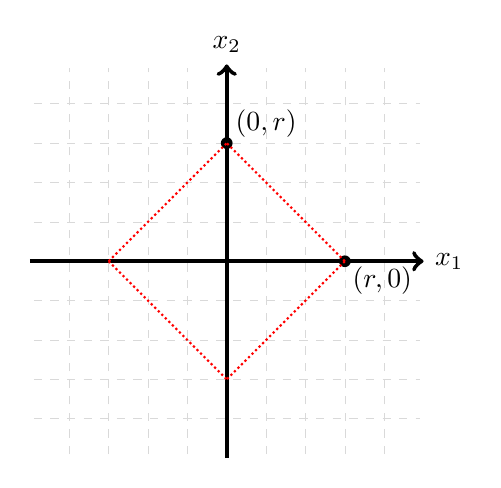
\begin{tikzpicture}[scale=0.5]
    \draw[help lines, color=gray!30, dashed] (-4.9,-4.9) grid (4.9,4.9);
    \draw[->,ultra thick] (-5,0)--(5,0) node[right]{$x_1$};
    \draw[->,ultra thick] (0,-5)--(0,5) node[above]{$x_2$};
    \node at (0,3) [circle,fill,inner sep=1.5pt]{};
    \node at (3,0) [circle,fill,inner sep=1.5pt]{};
    \node at (3.95,-0.5) {$(r,0)$};
    \node at (1,3.5) {$(0,r)$};
    
    \draw[densely dotted, thick, color=red] (3,0)--(0,3);
    \draw[densely dotted, thick, color=red] (-3,0)--(0,-3);
    \draw[densely dotted, thick, color=red] (-3,0)--(0,3);
    \draw[densely dotted, thick, color=red] (3,0)--(0,-3);
    \end{tikzpicture}}
    \subfloat[2-norm (Euclidean metric)]{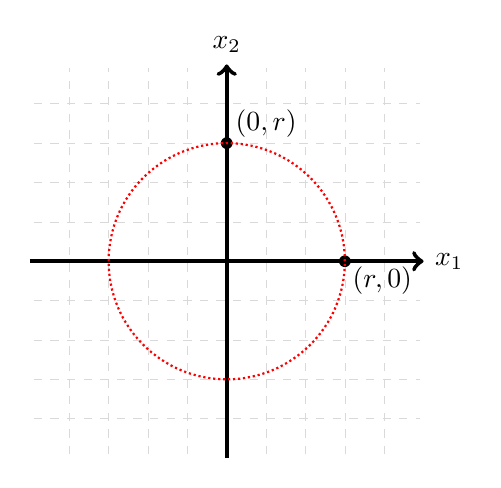
\begin{tikzpicture}[scale=0.5]
    \draw[help lines, color=gray!30, dashed] (-4.9,-4.9) grid (4.9,4.9);
    \draw[->,ultra thick] (-5,0)--(5,0) node[right]{$x_1$};
    \draw[->,ultra thick] (0,-5)--(0,5) node[above]{$x_2$};
    \node at (0,3) [circle,fill,inner sep=1.5pt]{};
    \node at (3,0) [circle,fill,inner sep=1.5pt]{};
    \node at (3.95,-0.5) {$(r,0)$};
    \node at (1,3.5) {$(0,r)$};
    
    \draw[densely dotted,thick, color = red] (0,0) circle [radius=3];
    \end{tikzpicture}}
    \subfloat[$\infty$-norm]{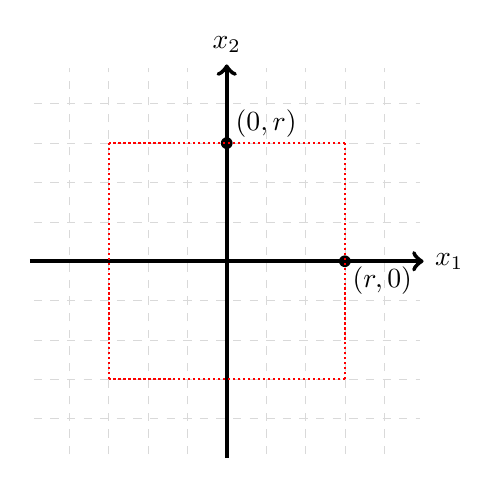
\begin{tikzpicture}[scale=0.5]
    \draw[help lines, color=gray!30, dashed] (-4.9,-4.9) grid (4.9,4.9);
    \draw[->,ultra thick] (-5,0)--(5,0) node[right]{$x_1$};
    \draw[->,ultra thick] (0,-5)--(0,5) node[above]{$x_2$};
    \node at (0,3) [circle,fill,inner sep=1.5pt]{};
    \node at (3,0) [circle,fill,inner sep=1.5pt]{};
    \node at (3.95,-0.5) {$(r,0)$};
    \node at (1,3.5) {$(0,r)$};
    
    \draw[densely dotted, thick, color=red] (3,-3) --(3,3);
    \draw[densely dotted, thick, color=red] (3,3) --(-3,3);
    \draw[densely dotted, thick, color=red] (-3,-3) --(-3,3);
    \draw[densely dotted, thick, color=red] (3,-3) --(-3,-3);
    \end{tikzpicture}}
    \caption{$B_r(0)$ for different metrics}
    \label{fig:open_ball}
\end{figure}

\end{example}

\begin{definition}[Open and closed sets]
Let $(X,d)$ be a metric space. 
\begin{itemize}
    \item A set $U \subseteq X$ is \emph{open} if for every $x \in U$ there exists $\epsilon>0$ such that $B_\epsilon(x) \subseteq U$.
    \item A set $F \subseteq X$ is \emph{closed} if $F^c:= X\setminus F$ is open.
\end{itemize}
\end{definition}

We note that $\emptyset$ and $X$ are both open and closed! 

\vspace{1em}

\begin{proposition}
\label{prop:open_sets}
Let $(X,d)$ be a metric space. 
 \begin{enumerate}
     \item[(i)] Let $A_1,A_2\subseteq X$. If $A_1$ and $A_2$ are open, then $A_1 \cap A_2$ is open.
     \item[(ii)] If $A_i \subseteq X$, $i \in I$ are open, then $\cup_{i\in I} A_i$ is open.
 \end{enumerate}
\end{proposition}
\begin{proof}
(i) Since $A_1$ is open, for each $x \in A_1$, there exists an $\epsilon_1 > 0$ such that $B_{\epsilon_1}(x) \subseteq  A_1$. Since $A_2$ is open, for each $x \in A_2$, there exists an $\epsilon_2 > 0$ such that $B_{\epsilon_2}(x) \subseteq A_2$. Let $x \in A_1 \cap A_2$. Choose $\epsilon = \min\{\epsilon_1,\epsilon_2\}$. Then  $B_{\epsilon}(x) \subseteq A_1 \cap A_2$ as required. 

(ii) Let $x\in \cup_{i\in I} A_i$. Then there exists $i \in I$ such that $x \in A_i$, and since $A_i$ is open there exists $\epsilon>0$ such that $B_\epsilon(x) \subseteq  A_i$. Since $A_i \subseteq \cup_{i\in I} A_i$, we are done.
\end{proof}

Using DeMorgan, we immediately have the following corollary:
\begin{corollary}
\label{cor:closed_sets}
Let $(X,d)$ be a metric space. 
 \begin{enumerate}
     \item[(i)] Let $A_1,A_2\subseteq X$. If $A_1$ and $A_2$ are closed, then $A_1 \cup A_2$ is closed.
     \item[(ii)]  If $A_i \subseteq X$, $i \in I$ are closed, then $\cap_{i\in I} A_i$ is closed.
 \end{enumerate}
\end{corollary}

\begin{definition}[Interior and closure]
Let $A\subseteq X$ where $(X,d)$ is a metric space. 
\begin{itemize}
    \item The \emph{closure} of $A$ is  $\overline A :=\{x \in X: \forall \epsilon > 0 \; B_\epsilon(x) \cap A \neq \emptyset \}$
    \item The \emph{interior} of $A$ is  $\interior A :=\{x \in X: \exists \epsilon > 0 \text{ s.t. } B_\epsilon(x) \subseteq A \}$
    \item The \emph{boundary} of $A$ is $\partial A := \{ x \in X: \forall \epsilon > 0, \, B_\epsilon(x) \cap A \neq \emptyset \text{ and }  B_\epsilon(x) \cap A^c \neq \emptyset\}$
\end{itemize}
\end{definition}
The closure of a set is the smallest closed set that contains it while the interior of a set is the largest open set contained by it.

\begin{example}
Let $X = (a, b] \subseteq \R$ with the ordinary (Euclidean) metric. Then $\overline X = [a,b]$, $\interior X = (a,b)$ and $\partial X = \{a,b\}$.
\end{example}

\begin{proposition}
 Let $A\subseteq X$ where $(X,d)$ is a metric space. Then $\interior A = A \setminus \partial A$.
\end{proposition}
\begin{proof}
First, we show $\interior A\subseteq A \setminus \partial A$. Let $x \in \interior A$. Then by definition $\exists \epsilon > 0 \text{ s.t. } B_\epsilon(x) \subseteq A$. Clearly $x \in A$ and also $\exists \epsilon > 0$ such that $B_\epsilon(x) \cap A^c = \emptyset$. Thus by definition, $x \notin \partial A$. Thus $x \in A \setminus \partial A$.

Next, we show $A \setminus \partial A \subseteq \interior A$. Let $x \in A \setminus \partial A$. Then $x \in A$ and $x \notin \partial A$. The latter means that $\exists \epsilon > 0$ such that $B_\epsilon(x) \cap A = \emptyset$ or  $B_\epsilon(x) \cap A^c = \emptyset$. Since $x \in A$, $x \in B_\epsilon(x) \cap A$ for any $\epsilon > 0$, so the former cannot be true. Therefore $\exists \epsilon > 0$ such that $B_\epsilon(x) \cap A^c = \emptyset$, i.e. $B_\epsilon(x) \subseteq A$. Thus $x \in \interior A$.
\end{proof}

\subsection{Sequences}

\begin{definition}
Let $(X,d)$ be a metric space. A \emph{sequence} is an ordered list of points $x_n$, $n\in\N$, in $X$, denoted $(x_n)_{n \in \N}$. We say that a sequence $(x_n)_{n \in \N}$ \emph{converges} to a point $x \in X$ if 
\begin{equation*}
    \forall \epsilon > 0 \, \exists \, n_\epsilon \in \N \text{ s.t. } d(x_n,x) < \epsilon \text{ for all } n \geq n_\epsilon .
\end{equation*}
\end{definition}

\begin{proposition}
\label{prop:closure_limit}
Let $(X, d)$ be a metric space, and let $A \subseteq X$. Then $\overline A$ is equal to the set of points in $X$ which are limits of a sequence in $A$.
\end{proposition}

\begin{proof}
Let $x \in \overline A$. Then by definition, for every $\epsilon > 0$, $B_\epsilon(x) \cap A \neq \emptyset$. In particular this is true for $\epsilon = 1/n$. Thus, for any $n \in N$, we can choose an $x_n \in A$ such that $x_n \in B_{1/n}(x)$, which means $d(x,x_n) < \frac{1}{n}$ by the definition of an open ball. Since $1/n$ decreases monotonically to zero, we must have $x_n \to x$.

Let $x \in X$ be the limit of a sequence $(x_n)_{n \in \N} \in A$. Then for $\epsilon > 0$, $\exists \, n_\epsilon \in \N$ such that $d(x_n,x) < \epsilon$ for all $n \geq n_\epsilon$. This means $x_n \in B_\epsilon(x)$, and since $x_n \in A$, $B_\epsilon(x) \cap A \neq \emptyset$. Thus $x \in \overline A$.
\end{proof}

Combining this result with the fact that $A \subseteq X$ is closed if and only if $A = \overline A$ (exercise), gives the following useful way to characterize closed sets. 

\begin{corollary}
\label{cor:closed_converge}
A set $F \subseteq X$, where $(X, d)$ is a metric space, is closed if and only if every sequence in $F$ which converges in $X$ converges to a point in $F$.
\end{corollary}

We also define a concept related to the closure of a set: a cluster or accumulation point.

\begin{definition}
Let $(X,d)$ be a metric space and $A \subseteq X$. A point $x \in X$ is a \emph{cluster point} of $A$ (also called accumulation point) if for every $\epsilon >0$, $B_\epsilon(x)$ contains infinitely many points in $A$.
\end{definition}


\begin{proposition}
\label{prop:cluster_seq}
 $x \in X$ is a cluster point of $A \subseteq X$ where $(X,d)$ is a metric space if and only if there exists a sequence of points $x_n \in A$, $n \in \N$, such that $x_n \to x$.
\end{proposition}

\begin{proof}
($\Leftarrow$) Suppose there exists a sequence $(x_n)_{n \in N}$ in $A$ such that $x_n \to x$. Then for every $\epsilon >0$, by the definition of a convergent sequence, $B_\epsilon(x)$ contains infinitely many elements of the sequence $x_n$ (in particular, $\exists n_0 \in \N$ such that $x_n \in B_\epsilon(x)$ for all $n \geq n_0$). Since each $x_n \in A$, $x$ is a cluster point of $A$.

($\Rightarrow$) Suppose $x$ is a cluster point of $A$. Then for any $\epsilon > 0$, $\exists x_\epsilon \in A$ such that $x_\epsilon \in B_\epsilon(x)$. In particular, take $\epsilon = 1/n$. Then $\exists x_n \in A$ such that $x_n\in B_{1/n}(x)$. By construction, such $x_n$ form a sequence in $A$ that converges to $x$. 

\end{proof}

Combining \cref{prop:closure_limit} and \cref{prop:cluster_seq} gives the following: 

\begin{corollary}
For $A \subseteq X$, $(X,d)$ a metric space, we have $\overline{A} = A \cup \{x \in X : x \text{ is a cluster point of }A \}$.
\end{corollary}

\subsubsection{Cauchy sequences}

\begin{definition}[Cauchy sequence]
Let $(X,d)$ be a metric space. A sequence denoted $(x_n)_{n \in \N} \in X$ is called a \emph{Cauchy sequence} if
\begin{equation*}
    \forall \epsilon >0  \; \exists \, n_\epsilon \in \N \text{ s.t. } d(x_n,x_m) < \epsilon \text{ for all } n,m \geq n_\epsilon .
\end{equation*}
\end{definition}

\begin{proposition}
\label{prop:converge_means_Cauchy}
Let $(X, d)$ be a metric space, and let $(x_n)_{n\in\N}$ be a convergent sequence in $X$. Then  $(x_n)_{n\in\N}$ is Cauchy.
\end{proposition}

\begin{proof}
Let $\epsilon > 0$ be arbitrary. Let $(x_n)_{n\in\N}$ be a convergent sequence in a metric space $(X,d)$. Then there exists $n_\epsilon \in \N$ such that $d(x_n,x) < \frac{\epsilon}{2}$ for all $n \geq n_\epsilon$. Then for $n,m \geq n_\epsilon$, using the triangle inequality we have
\begin{equation*}
    d(x_n,x_m) \leq  d(x_n,x) +  d(x,x_m) < \frac{\epsilon}{2} + \frac{\epsilon}{2} = \epsilon .
\end{equation*}
Thus $(x_n)_{n\in\N}$ is Cauchy.
\end{proof}

\begin{definition}
A metric space where every Cauchy sequence converges (to a point in the space) is called \emph{complete}.
\end{definition}

In addition, a normed space that is complete with respect to the metric induced by the norm is called a \emph{Banach space}. $\R^n$ with the Euclidean distance is complete (and is, in fact, a Banach space). 
%Note that this form of completeness is slightly weaker than the completeness mentioned in \cref{ax: completeness}, however, we will not go in to detail. 

\begin{proposition}[{\cite[Proposition 2.4.5]{tastetopology}}]
\label{prop:closed_subset_complete}
Let $(X, d)$ be a metric space, and let $Y\subseteq X$.
\begin{enumerate}
    \item[(i)] If $X$ is complete and if $Y$ is closed in $X$, then $Y$ is complete.
    \item[(ii)] If $Y$ is complete, then it is closed in $X$.
\end{enumerate}
\end{proposition}

\begin{proof}
(i) Let $X$ be a complete metric space and $Y$ be a closed subset of $X$. Let $(x_n)_{n\in\N}$ be a Cauchy sequence in $Y$. Since $Y \subseteq X$, $(x_n)_{n\in\N}$ is also a Cauchy sequence in $X$. Therefore $(x_n)_{n\in\N}$ converges to an $x \in X$ since $X$ is complete. But since $Y$ is closed, by \cref{prop:closure_limit}, we must have $x \in Y$. Therefore $Y$ is complete.

(ii) Let $(X, d)$ be a metric space and let $Y\subseteq X$ be complete. Let $(y_n)_{n\in\N}$ be a sequence in $Y$ that converges to some point $y \in X$.  By \cref{prop:converge_means_Cauchy},  $(y_n)_{n\in\N}$ is Cauchy in $X$ and therefore also in $Y$. Since $Y$ is complete, $(y_n)_{n\in\N}$ converges to a point $y' \in Y$. Since sequences in metric spaces converge to unique points (see exercises), $y=y'$. Thus $Y$ is closed by \cref{cor:closed_converge}.
\end{proof}

\subsubsection{Subsequences}

\begin{definition}
Let $(x_n)_{n \in \N}$ be a sequence in a metric space $(X,d)$. Let $(n_k)_{k \in \N}$ be a sequence of natural numbers with $n_1 < n_2 < \cdots$. The sequence $(x_{n_k})_{k \in \N}$ is called a \emph{subsequence} of $(x_n)_{n \in \N}$. If $(x_{n_k})_{k \in \N}$ converges to $x \in X$, we call $x$ a \emph{subsequential limit}.
\end{definition}

\begin{example}
The sequence $\left((-1)^n\right)_{n \in \N}$ diverges but the subsequences $\left((-1)^{2n}\right)_{n \in \N}$ and $\left((-1)^{2n-1}\right)_{n\in \N}$ converge to subsequential limits 1 and $-1$, respectively.
\end{example}

\begin{proposition}
A sequence $(x_n)_{n \in \N}$ in a metric space $(X,d)$ converges to $x \in X$ if and only if every subsequence of $(x_n)_{n \in \N}$  also converges to $x$.
\end{proposition}
\begin{proof}
($\Leftarrow$) If every subsequence of $(x_n)_{n \in \N}$ converges to $x \in X$, then  $(x_n)_{n \in \N}$ must converge to it as well, since a sequence is a subsequence of itself. 

($\Rightarrow$) Suppose $(x_n)_{n \in \N}$ converges to $x \in X$ and let $(x_{n_k})_{k \in \N}$ be an arbitrary subsequence of $(x_n)_{n \in \N}$. Let $\epsilon > 0$ be arbitrary. There exists $n_\epsilon \in \N$ such that $d(x_n,x) < \epsilon$ for all $n \geq n_\epsilon$. Choose $k_\epsilon$ such that $n_{k_\epsilon} \geq n_\epsilon$, which must exist since $(n_k)_{k\in\N}$ is strictly increasing. Then for all $k \geq k_\epsilon$, $d(x_{n_k},x) < \epsilon$. Thus $(x_{n_k})_{k \in \N}$ converges to $x$.
\end{proof}


\subsection{Continuity}

\begin{definition}
Let $(X,d_X)$ and $(Y,d_Y)$ be metric spaces, let $x_0 \in X$, and let $f:X\to Y$. $f$ is \emph{continuous} at $x_0$ if for every sequence $(x_n)_{n\in\N}$ in $X$ that converges to $x_0$, we have $\lim_{n\to\infty}f(x_n)=f(x_0)$.
We say that $f$ is \emph{continuous} if it is continuous at every point in $X$.
\end{definition}

\begin{theorem}[{\cite[Theorem 2.3.7.]{tastetopology}}]
\label{thm:cont_equiv}
Let $(X,d_X)$ and $(Y,d_Y)$ be metric spaces, let $x_0 \in X$, and let $f:X\to Y$. The following are equivalent:
\begin{enumerate}
    \item[(i)] $f$ is continuous at $x_0$
    \item[(ii)] for all $\epsilon>0$, there exists $\delta > 0$ such that $d_Y(f(x),f(x_0))) < \epsilon$ for all $x \in X$ with $d_X(x,x_0) < \delta$
    \item[(iii)] for each $\epsilon>0$, there is $\delta > 0$ such that $B_\delta(x_0) \subseteq f^\inv (B_\epsilon(f(x_0)))$
\end{enumerate}
\end{theorem}

\begin{proof}
(i) $\Rightarrow$ (ii) We prove the contrapositive. Assume
\begin{equation}
\label{star1} 
\exists \epsilon_0 \text{ such that } \forall \delta > 0 \text{ there exists an } x_\delta \in X \text{ with } d_X(x_\delta,x_0) < \delta \text{ and } d_Y(f(x_\delta),f(x_0))) \geq \epsilon_0
\tag{$\star$}
\end{equation}
We need to find a sequence in $X$ that converges to  $x_0$ but the sequence of images does not converge. Let's construct such a sequence. 

Let $\delta=\frac{1}{n}$ in \eqref{star1} for $n \in \N$. Then we can pick a sequence $x_n := x_{1/n}$ given by \eqref{star1} which converges to $x_0$. However, for each $n \in \N$, we have $d_Y(f(x_n),f(x_0))) \geq \epsilon_0$, so we cannot have $\lim_{n\to\infty}f(x_n)=f(x_0)$.

(ii) $\Rightarrow$ (iii) Follows from the definitions of the pre-image and open balls. 

(iii) $\Rightarrow$ (i) Let $(x_n)_{n\in\N}$ be a sequence in $X$ that converges to $x_0$. Let $\epsilon > 0$. Then by (iii), there exists $\delta > 0$ such that $B_\delta(x_0) \subseteq f^\inv (B_\epsilon(f(x_0)))$, i.e. if $x$ is such that $d_X(x,x_0) < \delta$, then $x$ is such that  $d_Y(f(x),f(x_0)) < \epsilon$. By the definition of convergence, there exists an $N \in \N$ such that $d(x_n,x_0)< \delta$ for all $n \geq N$. Then by (iii), $d(f(x_n),f(x_0))< \epsilon$ for all $n \geq N$. Thus $\lim_{n\to\infty}f(x_n)=f(x_0)$.
\end{proof}

\begin{corollary}
\label{cor:open_closed}
Let $(X,d_X)$ and $(Y,d_Y)$ be metric spaces and let $f:X\to Y$. The following are equivalent:
\begin{enumerate}
    \item[(i)] $f$ is continuous
    \item[(ii)] if $U \subseteq Y$ is open, then $f^\inv(U)$ is open
    \item[(iii)] if $F \subseteq Y$ is closed, then $f^\inv(F)$ is closed
\end{enumerate}
\end{corollary}

\textit{Note: the following proof uses the following results, which you may wish to prove as an exercise using techniques from the set theory section if they are not clear to you: Let $X$ and $Y$ be sets and $f:X \to Y$. Let $A,B \subseteq Y$. Then 
\begin{enumerate}
\item $A \subseteq B$ $\implies$ $f^\inv(A) \subseteq f^\inv(B)$
\item $f^\inv(Y \setminus A) = X \setminus f^\inv(A)$
\end{enumerate}}

\begin{proof}
Let $(X,d_X)$ and $(Y,d_Y)$ be metric spaces and let $f:X\to Y$.

(i) $\Rightarrow$ (ii): Suppose $f$ is continuous (on every point in $X$) and let $U \subseteq Y$ be open. Let $x \in f^\inv(U)$, then $f(x) \in U$, and since $U$ is open, there exists $\epsilon_0 > 0$ such that $B_{\epsilon_0}(f(x)) \subseteq U$. By \cref{thm:cont_equiv}(iii), there exists a $\delta_0 > 0$ such that $B_{\delta_0}(x) \subseteq f^\inv (B_{\epsilon_0}(f(x)))$. Since $B_{\epsilon_0}(f(x))) \subseteq U$, $f^\inv (B_{\epsilon_0}(f(x))) \subseteq f^\inv(U)$. Thus for each $x \in f^\inv(U)$, there exists $\delta_0$ such that $B_{\delta_0}(x) \subseteq f^\inv (B_{\epsilon_0}(f(x))) \subseteq f^\inv(U)$, so $f^\inv(U)$ is open.

(ii) $\Rightarrow$ (i): We want to prove that $f$ is continuous at every $x \in X$ using the definition from \cref{thm:cont_equiv}(iii), i.e. we must show that for $x \in X$, for each $\epsilon>0$, there is $\delta > 0$ such that $B_\delta(x) \subseteq f^\inv (B_\epsilon(f(x)))$. 

Let $x\in X$ and let $\epsilon > 0$ be arbitrary. Since $B_\epsilon(f(x))$ is an open set, by (ii), $f^\inv(B_\epsilon(f(x)))$ is also open. Since $x \in f^\inv(B_\epsilon(f(x)))$, there exists a $\delta > 0$ such that $B_\delta(x) \subseteq f^\inv(B_\epsilon(f(x)))$ by the definition of a set being open, so we are done.

(ii) $\Rightarrow$ (iii): Let $F \subseteq Y$ be closed. Then $Y \setminus F$ is open, so by (ii), $f^\inv(Y \setminus F)$ is open as well. Since $f^\inv(Y \setminus F) = X\setminus f^\inv(F)$, $f^\inv(F)$ is closed.

(iii) $\Rightarrow$ (ii) follows from the above, exchanging ``open'' and ``closed''.

\end{proof}


\begin{definition}
Let $(X,d_X)$ and $(Y,d_Y)$ be metric spaces and let $f:X\to Y$. 
\begin{itemize}
    \item $f$ is \emph{uniformly continuous} if for all $\epsilon>0$, there exists $\delta > 0$ such that for every $x_1,x_2\in X$ with $d_X(x_1,x_2) < \delta$, we have  $d_Y(f(x_1),f(x_2))) < \epsilon$ 
    \item $f$ is \emph{Lipschitz continuous} if there exists a $K > 0$ such that for every $x_1,x_2\in X$ we have  $d_Y(f(x_1),f(x_2))) \leq K d_X(x_1,x_2)$
\end{itemize}
\end{definition}

\begin{proposition}
Let $(X,d_X)$ and $(Y,d_Y)$ be metric spaces and let $f:X\to Y$. 
$$f \text{ is Lipschitz continuous } \Rightarrow \text{ f is uniformly continuous } \Rightarrow \text{ f is continuous}$$
\end{proposition}

The proof is left as an exercise. 

\begin{definition}
Let $(X,d)$ be a metric space and let $f:X \to X$. We say that $x^* \in X$ is a \emph{fixed point} of $f$ if $f(x^*) = x^*$.
\end{definition}

\begin{definition}
Let $(X,d)$ be a metric space and let $f:X \to X$. $f$ is a \emph{contraction} if there exists a constant $k \in [0,1)$ such that for all $x,y \in X$, $d(f(x),f(y))) \leq k d(x,y)$.
\end{definition}

Observe that a function is a contraction if and only if it is Lipschitz continuous with constant $K < 1$.

\begin{theorem}
Suppose that $f : X \to X$ is a contraction and the metric space $X$ is complete. Then $f$ has a unique fixed point $x^*$.
\end{theorem}

We omit the proof here; see \cite[p.240]{realanalysis} for the proof as well as more details on how to find the fixed point.

\begin{example}
Let $f:\left[-\frac{1}{3},\frac{1}{3}\right] \to \left[-\frac{1}{3},\frac{1}{3}\right]$ be defined by the mapping $x \mapsto x^2$. Assume we use the standard Euclidean metric, $d(x,y) = |x-y|$. $f$ has a unique fixed point because $\left[-\frac{1}{3},\frac{1}{3}\right]$ is a complete metric space (see \cref{prop:closed_subset_complete}) and $f$ is a contraction with Lipschitz constant 2/3.

To see that it is a contraction, let $x,y \in \left[-\frac{1}{3},\frac{1}{3}\right]$. Then
\begin{equation*}
   |x^2 - y^2| = |x+y| |x-y| \leq \frac{2}{3} |x-y|. 
\end{equation*}
\end{example}

\subsection{Equivalence of metrics}

\begin{definition}[Equivalent metrics]
Two metrics $d_1$ and $d_2$ on a set $X$ are \emph{equivalent} if the identity maps from $(X,d_1)$ to $(X,d_2)$ and from $(X,d_2)$ to $(X,d_1)$ are continuous. 
\end{definition}

The following result follows from the definition and \cref{cor:open_closed}:

\begin{proposition}
Two metrics $d_1$, $d_2$ on a set $X$ are equivalent if and only if they have the same open sets or the same closed sets.
\end{proposition}

So, in a certain sense, equivalent metrics induce the same structure.

\begin{definition}
Two metrics $d_1$ and $d_2$ on a set $X$ are \emph{strongly equivalent} if for every $x,y\in X$, there exists constants $\alpha>0$ and $\beta>0$ such
\begin{equation*}
    \alpha d_1(x,y) \leq d_2(x,y) \leq \beta d_1(x,y).
\end{equation*}
\end{definition}

If two metrics are strongly equivalent then they are equivalent. The proof of this is part of the exercises. 

\begin{example}
We show that the Euclidean distance (induced by 2-norm) and the metric induced by the $\infty$-norm are equivalent on $\R^n$. 

\vspace{1em}
Let $\|x-y\|_2=\sqrt{\sum_{j=1}^n (x_j - y_j)^2}$ be the Euclidean metric and $\|x-y\|_\infty= \max_{j=1,\ldots,n} |x_j - y_j|$ be the metric induced by the $\infty$-norm. We have
\begin{equation*}
   \|x-y\|_2 = \sqrt{\sum_{j=1}^n (x_j - y_j)^2} \leq  \sqrt{ n \max_{j=1,\ldots,n} (x_j - y_j)^2}  = \sqrt{n} \max_{j=1,\ldots,n} |x_j - y_j| = \sqrt{n} \, \|x-y\|_\infty
\end{equation*}
and
\begin{equation*}
    \|x-y\|_\infty = \max_{j=1,\ldots,n} |x_j - y_j|  = \sqrt{\max_{j=1,\ldots,n} (x_j - y_j)^2} \leq \sqrt{\sum_{j=1}^n(x_j - y_j)^2}  = \|x-y\|_2  \, .
\end{equation*}
Thus the two metrics are strongly equivalent. 
\end{example}

\subsection{Extra properties of $\R$}

Using the definition of continuity in terms of $\epsilon$-balls and equipping $\R$ with the metric induced by the absolute value, i.e. $d(x,y) = \vert x- y\vert$ for $x,y\in \R$, we obtain the usual $\epsilon-\delta$ definition of continuity. Hence, a function $f\colon \R \to \R$ is continuous at $x_0\in \R$ if for all $\epsilon>0$ there exists a $\delta>0$ such that $\vert x_0-y\vert <\delta$ implies $\vert f(x_0)-f(y)\vert<\epsilon$. Since $\R$ is also totally ordered we can also talk about left and right continuity, by separating $B_\epsilon(x) = (x-\epsilon, x+ \epsilon) = (x-\epsilon, x] \cup [x, x+\epsilon)$.

\begin{definition} Let $f\colon \R \to \R$.
\begin{itemize}
    \item $f$ is \emph{left continuous} at $x_0\in \R$ if for all $\epsilon >0$ there exists a $\delta>0$, such $\vert f(x_0)-f(x)\vert<\epsilon$ whenever $ x_0-\delta <x<x_0$.
    \item $f$ is \emph{right continuous} at $x_0\in \R$ if for all $\epsilon >0$ there exists a $\delta>0$, such $\vert f(x_0)-f(x)\vert<\epsilon$ whenever $x_0<x<x_0+\delta$.
\end{itemize}
We say that $f$ is left continuous if is left continuous at all points in the domain, and similar for right continuous.
\end{definition}

Similar to the ordinary sense of continuity, one can describe left and right continuity in terms of sequences. 

\begin{proposition}
 A function $f\colon \R \to \R$ is continuous if and only if it is left and right continuous. 
\end{proposition}

This proof essentially follows from the definitions:
\begin{proof}
($\Leftarrow$) Suppose $f:\R \to \R$ is both right and left continuous. Let $\epsilon > 0$ be arbitrary. Then by the definition of left continuous, there exists a $\delta_1>0$, such $\vert f(x_0)-f(x)\vert<\epsilon$ whenever $ x_0-\delta_1 <x<x_0$, and by the definition of right continuous, there exists a $\delta_2>0$, such $\vert f(x_0)-f(x)\vert<\epsilon$ whenever $x_0<x<x_0+\delta_2$.

Let $\delta = \min\{\delta_1,\delta_2\}$. Let $x \in \R$ such that $\vert x_0-x\vert <\delta$. Then $x_0- \delta < x < x_0 + \delta$. 

Case 1: Suppose $x < x_0$. Then $x_0- \delta_1 < x <x_0$, so $\vert f(x_0)-f(x)\vert<\epsilon$, so $f$ is continuous.

Case 2: Suppose $x > x_0$. Then $x_0 < x < x_0 + \delta_2$, so $\vert f(x_0)-f(x)\vert<\epsilon$, so $f$ is continuous.

If $x=x_0$, the result is trivial, so we conclude that $f$ is continuous.

($\Rightarrow$) Let $f:\R \to \R$ be continuous. Then for every $\epsilon >0$, $\exists \delta_0 > 0$ such that when $x$ is such that $|x - x_0| < \delta$, then $|f(x) - f(x_0)| < \epsilon$.

For $\epsilon > 0$ arbitrary, take $\delta_0$ from the definition of $f$ being continuous.  Take $x \in \R$ such that $x_0 < x < x_0 + \delta_0 $. Then $x_0 - \delta_0 < x < x_0 + \delta_0 $, which implies $|x - x_0| < \delta_0 $. Thus  $|f(x) - f(x_0)| < \epsilon$, so $f$ is right-continuous.

The proof for left-continuity is similar. 
\end{proof}

Using the least upper bound property of sets, we can introduce the concepts of limit inferior and limit superior as the limit of infima and suprema when we view the sequence as a set. First, we recall what it means for a sequence to be bounded.

\begin{definition}
Let $(x_n)_{n\in \N}$ be a sequence in $\R$. We call $(x_n)_{n\in \N}$ \emph{bounded} if there exists an $M > 0$ such that $\vert x_n\vert<M$ for all $n\in \N$.
\end{definition}

This definition is equivalent to the set of sequence elements being bounded in the metric space setting. Similarly, one can talk about a sequence being bounded above or below in the order theoretic setting (see \cref{sec:ordered_sets}), by looking at the set of sequence elements. The next theorem is useful.

\begin{theorem}[Monotone convergence theorem]
\label{thm:mon_conv}
\textcolor{white}{skip}
\begin{itemize}
\item[(i)] Suppose $(x_n)_{n\in \N}$ is an increasing sequence, i.e. $x_n\leq x_{n+1}$ for all $n\in \N$ and that it is bounded above. Then the sequence converges. Furthermore, $\lim_{n\to \infty} x_n = \sup_{n\in \N} x_n$, where $\sup_{n\in \N} x_n := \sup\{x_n \; \colon \; n\in \N\}$.
\item[(ii)] $(x_n)_{n\in \N}$ is a decreasing sequence, i.e. $x_n\geq x_{n+1}$ for all $n\in \N$, which is bounded below. Then the sequence converges and $\lim_{n\to \infty} x_n = \inf_{n\in \N} x_n := \inf\{x_n \; \colon \; n\in \N\}$. 
\end{itemize}
\end{theorem}

The proof is omitted. We call increasing or decreasing sequences monotone, hence the theorem name.

If the sequence is increasing but not bounded above, then $\lim_{n\to \infty} x_n = \infty$, and if it is decreasing but not bounded below, then $\lim_{n\to \infty} x_n = -\infty$.

 We would like to use the monotone convergence theorem for arbitrary sequences. We do so by building an increasing sequence (or decreasing) sequence from an arbitrary one. First, we recall some facts about infima and suprema and introduce the convention that $\sup A = \infty$ if $A\subseteq \R$ is not bounded above and $\inf A= -\infty$ if $A$ is not bounded below.

\begin{lemma}\label{lem:inf_sup_inequality}
If $A \subseteq B \subseteq \R$ is non-empty, then $\inf A \leq \sup A$, $\sup A \leq \sup B$, and $\inf A \geq \inf B$.
\end{lemma}
The proof of this follows from the definition of greatest lower and least upper bound. 

\begin{definition}
Let $(x_n)_{n\in \N}$ be a sequence in $\R$. We define the \emph{limit superior} of $(x_n)_{n\in \N}$ as 
$$\limsup_{n\to \infty} x_n: = \lim_{n\to \infty} \sup_{k\geq n} x_k.$$ 
Similarly we define  the \emph{limit inferior} of $(x_n)_{n\in \N}$ as 
$$\liminf_{n\to \infty} x_n: = \lim_{n\to \infty} \inf_{k\geq n} x_k.$$
\end{definition}

\begin{proposition}\label{prop:limsup_monotonicity}
Let $(x_n)_{n \in \N}$ be a sequence in $\R$.
\begin{itemize} 
\item The sequence of suprema, $s_n = \sup_{k\geq n} x_k$, is decreasing and the sequence of infima, $i_n = \inf_{k\geq n} x_k$, is increasing.
\item The limit superior and the limit inferior of a bounded sequence always exist and are finite.
\end{itemize}
\end{proposition}
\begin{proof}
The first part is true by Lemma 3.45. The second the follows by the Monotone Convergence Theorem.
\end{proof}

Conceptually, we can think of the limit superior as the greatest cluster point of a sequence, and of the limit inferior as the least.
If the sequence $(x_n)_{n\in \N}$ is not bounded above, then $\limsup_{n\to \infty} x_n = \infty$. Similarly, if the sequence $(x_n)_{n\in \N}$ is not bounded below, then $\liminf_{n\to \infty} x_n = -\infty$. This is in line with our convention that $\sup A = \infty$, if $A$ is not bounded above and $\inf A = -\infty$, if $A$ not bounded below. 

\begin{theorem}
Let $(x_n)_{n\in \N}$ be a sequence in $\R$. Then the sequence converges to $x\in \R$ if and only if $\limsup_{n\to \infty} x_n= x =\liminf_{n\to \infty} x_n$.
\end{theorem}

\begin{proof}
For convenience, denote $i_n := \inf_{k\geq n} x_k$ and $s_n :=  \sup_{k\geq n} x_k$ for $n\in \N$.


($\Rightarrow$) Suppose $\lim_{n\to \infty} x_n = x\in \R$ and let $\epsilon>0$. Since the sequence converges, there exists an $N\in \N$ such that $\vert x-x_n\vert <\epsilon$, i.e. $x-\epsilon<x_n<x+\epsilon$, for all $n\geq N$. 

In particular, $x-\epsilon<x_n$ for all $n\geq N$, so $x-\epsilon$ is a lower bound for the set $\{x_n \colon n\geq N\}$. Therefore $x-\epsilon\leq i_N$. 

Similarly, since $x_n<x - \epsilon$ for all $n\geq N$, $x+\epsilon$ is an upper bound for the set $\{x_n \colon n\geq N\}$. Therefore $s_N \leq x + \epsilon$. 

By \cref{prop:limsup_monotonicity} the sequence of infima is increasing and by the Monotone Convergence Theorem, its limit is given by the supremum of the sequence. Hence, we obtain 
$$x-\epsilon\leq i_N \leq \lim_{n \to \infty} i_n =  \liminf_{n\to \infty} x_n.$$ 

Similarly, since the sequence of suprema is decreasing and using the Monotone Convergence theorem again, we obtain 
$$\limsup_{n\to \infty} x_n\leq s_N<x+\epsilon.$$
Now observe that $\liminf_{n\to \infty} x_n\leq \limsup_{n\to \infty} x_n $, since $i_n\leq s_n$ for all $n\in \N$ by \cref{lem:inf_sup_inequality} (exercise: $x_n \leq y_n$ for all $n \in \N$ implies $\lim_{n\to \infty} x_n \leq \lim_{n\to \infty} y_n$). Thus we have
\begin{align*}
    x-\epsilon \leq \liminf_{n\to \infty}x_n \leq \limsup_{n\to \infty} x_n \leq x+\epsilon.
\end{align*}
Since this holds for any $\epsilon$, the desired result follows.

($\Leftarrow$) Now suppose $\limsup_{n\to \infty} x_n= x =\liminf_{n\to \infty} x_n$. We need to show that $\lim_{n\to\infty} x_n = x$. 

Let $\epsilon>0$. Then since $\limsup_{n\to \infty} x_n = \lim_{n\to \infty} s_n= x$, there exists an $N_1\in \N$ such that $\vert s_n - x\vert <\epsilon$ for all $n\geq N_1$. In particular, 
$$x_n<s_{N_1} < x+\epsilon \qquad \text{ for all } n\geq N_1.$$ 

Similarly, there exists $N_2\in \N$ such that $\vert i_n - x\vert <\epsilon$ for all $n\geq N_2$ giving 
$$x-\epsilon< i_{N_2} x_k< x_n  \qquad \text{ for all } n\geq N_2.$$ Hence, by setting $N= \max\{N_1,N_2\}$ we see $x-\epsilon < x_n < x+ \epsilon$ or equivalently $\vert x_n - x\vert < \epsilon$ for all $n\geq N$, which proves the result. 
\end{proof}

Note that we only talked about limit superior and limit inferior for real sequences. However, we can extend this easily to a sequence of functions $f_n \colon X \to \R$ by setting $f = \limsup_{n\to \infty } f_n$ to be the function defined pointwise by $f(x) = \limsup_{n\to \infty } (f_n (x)) $ and similar for the limit inferior. There also exists a set theoretic version in terms of unions and intersections which you will encounter in probability.

\subsection{Exercises}
\label{exercises:metric_spaces}
\begin{enumerate}
    \item Show that the infinity norm $||x||_\infty$, $x \in \R^n$, defined in \cref{p-norm} is a norm.
    \item Let $(X,d)$ be any metric space, and define $\tilde d: X \times X \to \R$ by 
    \begin{equation*}
        \tilde d(x,y) = \frac{d(x,y)}{1+d(x,y)}, \quad x,y \in X .
    \end{equation*}
    Show that $\tilde d$ is a metric on $X$.
    \item Let $X$ be a set and define $d\colon X \times X \to \R$ by $d(x,x) = 0$ and $d(x,y)=1$ for $x\neq y \in X$. Prove that $d$ is a metric on $X$. What do open balls look like for different radii $r>0$? What does an arbitrary open set look like?
    \item Following up on \cref{prop:open_sets} and \cref{cor:closed_sets}: Show that the infinite intersection of open sets may not be open and that the infinite union of closed sets may not be closed.
    \item Find the closure, interior, and boundary of the following sets using Euclidean distance:
    \begin{enumerate}
        \item[(i)] $\{(x,y)\in \R^2 : y < x^2 \} \subseteq \R^2$
        \item[(ii)]  $[0,1)\times[0,1) \subseteq \R^2$
        \item[(iii)] $\{0 \} \cup  \{1/n \colon n \in \N\} \subseteq \R$ 
    \end{enumerate}
    \item Prove the following: Let $(x_n)_{n\in\N}$ be a sequence in a metric space $(X,d)$ that converges to a point $x \in X$. Then $x$ is unique.
    \item Let $(x_n)_{n \in \N}$ and $(y_n)_{n \in \N}$ be sequences in $\R$ such that $x_n \to x$ and and $y_n \to y$, with $\alpha, x,y, \in \R$. 
    \begin{enumerate}
        \item[(i)] Show that $\alpha \, x_n \to \alpha \, x$.
        \item[(i)] Show that $x_n + y_n \to x + y$.
    \end{enumerate}
    \item Let $(x_n)$, $(y_n)$ be two convergent sequences in $\R$ such that $x_n \leq y_n$ for all $n \in \N$. Show that $\lim_{n\to \infty} x_n \leq \lim_{n\to \infty} y_n$.
    \item Show that discrete metric spaces (i.e. those with the metric from exercise 3) are complete. 
    \item Let $(X,d_X)$ and $(Y,d_Y)$ be metric spaces and let $f:X\to Y$. Prove that
$$f \text{ is Lipschitz continuous } \Rightarrow f \text{ is uniformly continuous } \Rightarrow f \text{ is continuous}.$$
Provide examples to show that the other directions do not hold.
    \item Show that the function $f(x) = \frac{1}{2} \left(x + \frac{5}{x} \right)$ has a unique fixed point on a subset of $(0,\infty)$. What is it? (Hint: you will have to restrict the interval in such a way that $f$ is a contraction.)
    \item Prove the following: If two metrics are strongly equivalent then they are equivalent.
    \item Let $(x_n)_{n\in N}$ be a sequence in $\R$. Show that $\lim_{n\to \infty} x_n = 0$ if and only if $\limsup_{n\to \infty} \vert x_n\vert = 0$.
\end{enumerate}

\subsection{References}
The content in this section comes mostly from \cite{tastetopology}. \cite{realanalysis} is used to supplement, and in particular the content on accumulation points and contractions comes from there. For lim sup and lim inf, see \cite{BasicAnalysis1}.
\newpage

\bibliographystyle{alphaurl} 
\bibliography{references}

\end{document}
